\section{Inlämning}
\subsection{Inlämning via Git}

Water tar emot inlämningar via Git. Det sker genom att studenten skriver ett commit-meddelande som innehåller strängen |\#submit| och därefter skickar data till Water med hjälp av Git kommandot git-push. Det går även att skicka data till Water utan att göra en inlämning.

Som en del av git-push-processen kommer Water att autentisera användaren. 

För att göra en git-push behöver användaren en sökväg.
Git-sökvägar i Water har följande form:

\begin{verbatim}
  courses/:course_id/lab_groups/:lab_group_number/labs/:lab_number.
\end{verbatim}

Kursen identifieras alltså av sitt databas-id, medan vi använder relativa nummer för de andra två. En student kan exempelvis ladda upp sitt arbete till Water för första gången genom att köra dessa kommandon:

\begin{verbatim}
  git init my-repo
  cd my-repo
  git remote add origin https://water.se/courses/1/lab_groups/1/labs/1 % fiktiv host
  touch README
  git add README
  git commit -m "Initial commit"
  git push origin master
  Username: my_cid
  Password: my_password  
\end{verbatim}

För att underlätta för en användare står ovanstånde kommandon uppradade i webbinterfacet. När en handledare eller laborationskamrater skall granska laborationen kan de också använda Git-interfacet för att hämta det senaste arbetet.

\begin{verbatim}
  git clone https://water.se/courses/1/lab_groups/1/labs/1
  Username: my_cid
  Password: my_password
\end{verbatim}

\subsection{Uppladdning och inlämning via webbgränssnittet}

\begin{figure}
  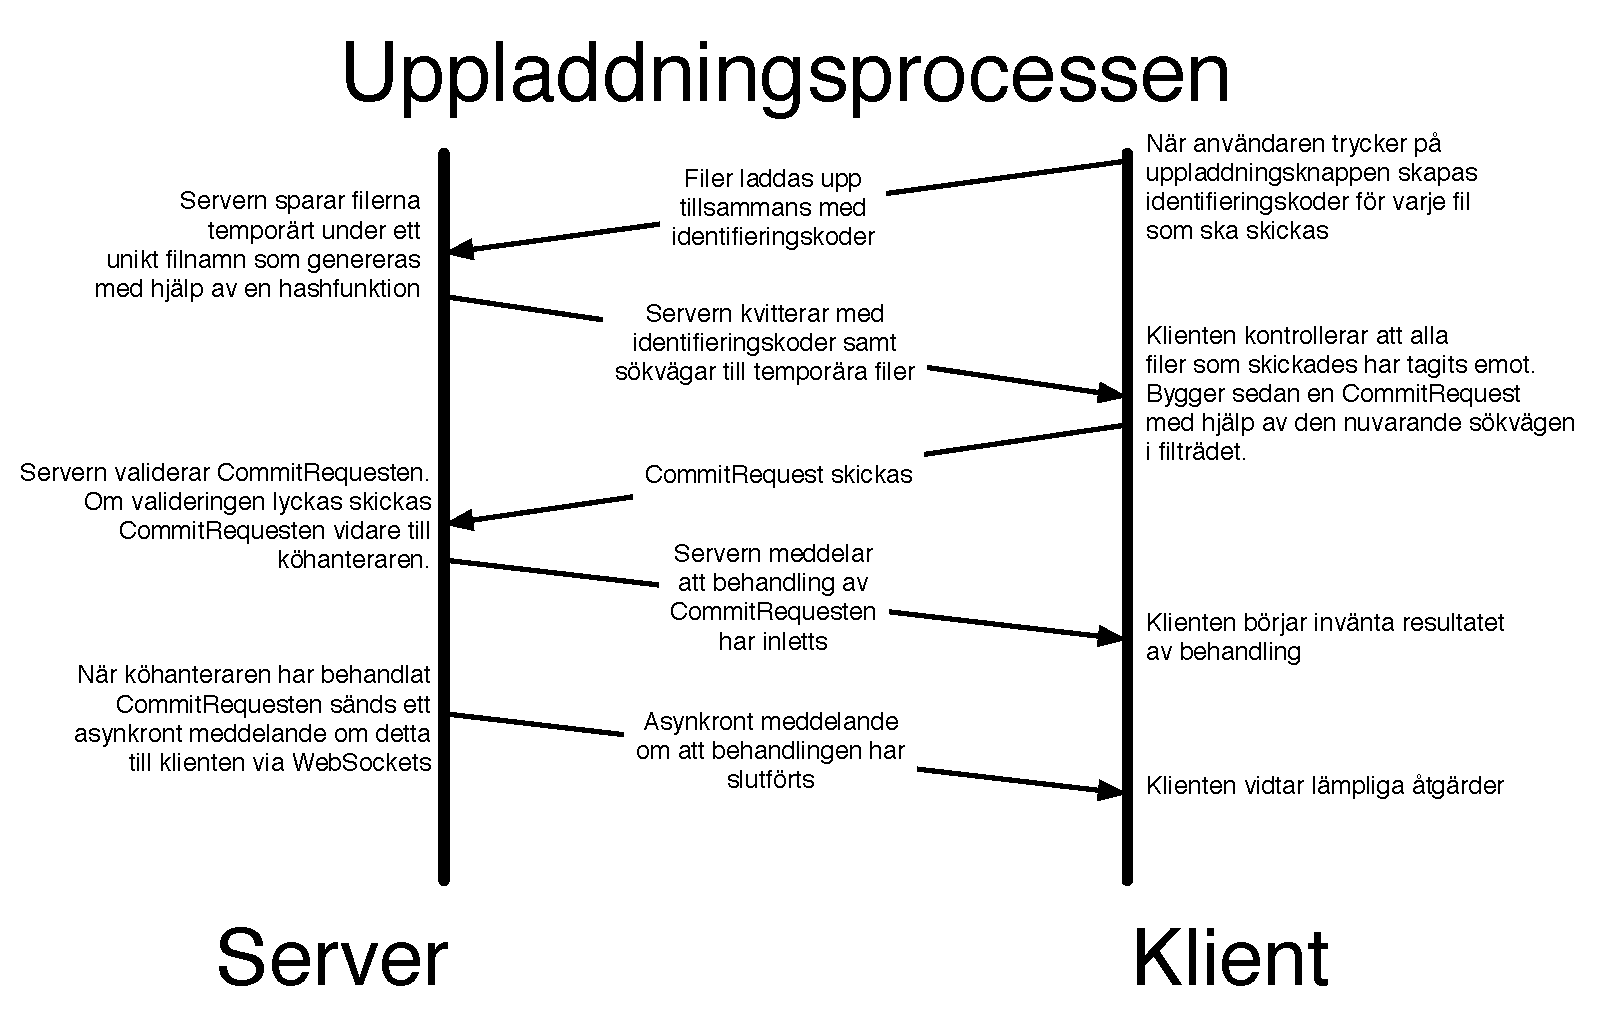
\includegraphics[width=15.0cm]{fig/misc/uppladdningsprocessen.pdf}             
  \caption[Uppladdningsprocessen]
  {Uppladdningsprocessen}
  \label{fig:uppladdning}
\end{figure}


Uppladdningsprocessen består av ett antal faser. Först laddas filerna upp. Därefter skickar klienten ett anrop som begär att filerna ska läggas till i ett repositorium. Servern svarar att processen har inletts och vidarebefordrar anropet till köhanteraren. När processen är klart får klienten ett asynkront meddelande om detta via WebSocket-servern. Se figur \ref{fig:uppladdning}

\subsubsection{Filerna laddas upp}

Javascriptbiblioteket JQuery-File-Upload används för att stöda uppladdning av flera filer genom ett enda anrop. 
Callbacks i JQuery-File-Upload används för att skicka med unika identifieringskoder för varje fil som laddas upp. Identifieringskoderna skapas med en enkel \emph{hashfunktion} som bygger på hashCode()-metoden för en sträng i Java.

Identifieringskoderna och filernas originalfilnamn lagras i en \emph{CommitRequest}-modell i klienten när filerna skickas. Servern svarar med en array där varje fil representeras av sin identifieringskod. På detta sätt får \emph{CommitRequest}-modellen ett kvitto på att uppladdningsprocessen är färdig. \emph{CommitRequest}-modellen delar upp kvitterade filer i lyckade och misslyckade uppladdningar. 

När alla filer är kvitterade tar \emph{CommitRequest}-modellen de filer vars uppladdning lyckades och konstruerar ett \emph{CommitRequest}-anrop till servern. Filernas sökvägar i Gitrepositoriet konstrueras med hjälp av trädvyns nuvarande sökväg, som lagras i BreadcrumbSet-modellen, samt originalfilnamnen som lagrades tillsammans med identifieringskoderna.
När uppladdningssidan hämtas lägger webbservern till Javascript-variabler i sidan. Variablerna innehåller en länk till det  repositorium som ska användas och namnet på den \emph{branch} som ska användas. \emph{CommitRequets}-modellen hämtar dessa och kan sedan skicka anropet.

\subsubsection{Filerna läggs till i Git}

Servern validerar \emph{CommitRequest}-anropet. Om valideringen lyckas skickas anropet vidare till köhanteraren och servern svarar till klienten att behandling av anropet har inletts. När klienten får detta meddelande låses webbgränsnittet.
När köhanteraren har behandlat anropet och lagt till filerna i Gitrepositoriet, skickas ett ansynkront meddelande om detta till klienten via SecureFaye och WebSocket-servern. Klienten kan då låsa upp gränssnittet och ladda om filträdet.

\subsection{Inlämningens livscykel}

För att implementera inlämningsuppgiftens livscykel har tillståndshantering implementerats i LabHasGroup-entiteten. LabHasGroup representerar kopplingen mellan en laboration och en grupp.
Tillstånden beskrivs som följer, se även illustration \ref{fig:cyk}:

\begin{figure}
  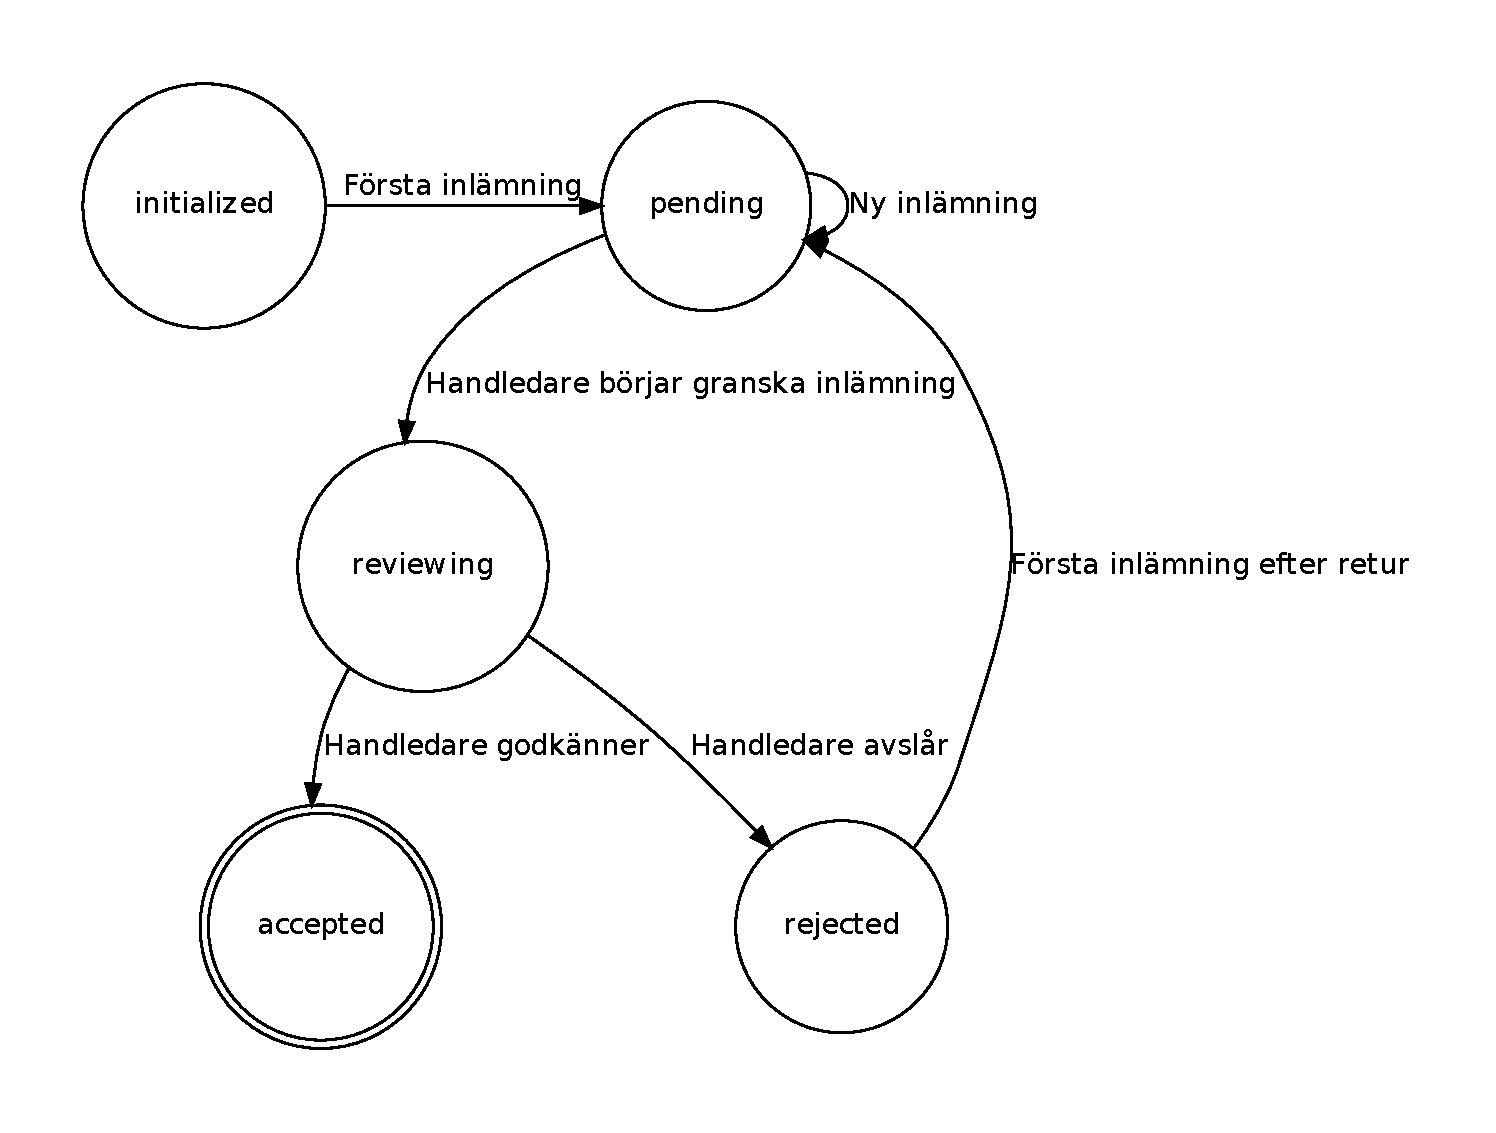
\includegraphics[width=15.0cm]{fig/labgroup/state-machine.pdf}             
  \caption[Inlämningsuppgiftens livscykel]
  {Inlämningens livscykel}
  \label{fig:cyk}
\end{figure}

\subsubsection{Initialized}

När en LabHasGroup skapas sätts objetet i tillståndet initalized. I detta tillstånd finns inga Submissions kopplade till entiteten.

\subsubsection{Pending}

När gruppen gör en inlämning skapas en Submission och LabHasGroup-entiteten övergår till tillståndet pending. Pending betyder att en inlämning är gjord, men att ingen handledare granskat laborationen.
Om en LabHasGroup befinner sig i pending kan dess senaste Submission uppdateras så att den pekar på ett nytt tillstånd i repositoriet.

\subsubsection{Reviewing}

Så snart en handledare har påbörjat granskningen en laboration övergår LabHasGroup-entiteten till tillståndet reviewing. I detta tillstånd är det inte möjligt att göra flera inlämningar

\subsubsection{Rejected och Accepted}

Efter granskning kan handledaren godkänna eller förkasta inlämningen. Om inlämningen är godkänd går LabHasGroup-entiteten över i tillståndet accepted. Inga fler inlämningar tas emot. Om inlämningen förkastas går entiteten över i tillståndet rejected. I rejected-tillståndet är det möjligt att göra en ny inlämning, varpå tillståndet övergår i pending.
